%++++++++++++++++++++++++++++++++++++++++
% Don't modify this section unless you know what you're doing!
\documentclass[letterpaper,12pt]{article}
\usepackage{tabularx} % extra features for tabular environment
\usepackage{amsmath}  % improve math presentation
\usepackage{graphicx} % takes care of graphic including machinery
\usepackage[margin=1in,letterpaper]{geometry} % decreases margins
\usepackage{cite} % takes care of citations
\usepackage[latin9]{inputenc}
\usepackage{lmodern} % for writing code
\usepackage{tikz}
\usetikzlibrary{positioning,shapes.geometric}
\usepackage{minted}


\usepackage[final]{hyperref} % adds hyper links inside the generated pdf file
\hypersetup{
	colorlinks=true,       % false: boxed links; true: colored links
	linkcolor=blue,        % color of internal links
	citecolor=blue,        % color of links to bibliography
	filecolor=magenta,     % color of file links
	urlcolor=blue         
}
\usepackage{xcolor}
%\usepackage[usenames,dvipsnames,svgnames,table]{xcolor}
%\let\oldtriangleleft\triangleleft
%\DeclareRobustCommand\bowtie{\mathrel\triangleright\joinrel\mathrel\oldtriangleleft}


%++++++++++++++++++++++++++++++++++++++++


\begin{document}

\title{Software Verification\\
Implementing a bounded model-checker}
\author{Ida Tucker}
\date{\today}
\maketitle

\begin{abstract}
The goal of this homework is to implement a bounded model-
checker based on a depth-first-search exploration of all the feasible paths
of the input program. Moreover, the SMT-solver Z3 will be used as an
execution engine to compute all the successive states along the explo-
ration. We will first present the global picture of it, then introduce a
few definition and semantics and, finally, list the steps you may follow
to implements the whole model-checking program.
\end{abstract}


\section{Implementation of Semantics.ml}
\paragraph{}
The \texttt{Semantics.ml} module translates the operators of the program into Z3 expressions in the integer theory module.
\subsection{Keeping track of formulas added to the Z3 expression}
\paragraph{}
In order to keep track of the formulas associated to each variable, a hashtable, global to the module, which is reset to zero for every new formula, is used. This hashtable \textit{\textcolor{blue}{ht}} binds the indexed program variables to the appropriate formula.
Seperate keys are added if the formula is asserting that a variable is non zero. These keys are of the form "\textit{x\$i non-zero}".
The hashtable has one additional key "\textit{guard}". If the program operation \textit{op} is a guard, the formula for the guard exists alongside the formulas added for each variable. Moreover we will only have one guard formula per operation.
\paragraph{}
Using a hashtable enables us to avoid the duplication of formulas associated to a given variable and to easily update them without having to check their existance. 
Thus the keys in the hashtable are:
\begin{itemize}
\item $\forall x \in X$,  \textcolor{purple}{x\$i}
\item $\forall x \in X$ such that we require $x \neq 0$, \textcolor{purple}{x\$inon-zero}
\item if \textit{op} is a guard, \textcolor{purple}{guard}
\end{itemize}

\subsection{Defining propositional formulas}
\paragraph{}
Now we have established how to keep track of the added formulas, let us see how they are built.
The commands are our program operations. In order to transform the program operation into a list of formulas we first need to determine what command is being applied.
Therefore, the \textcolor{blue}{formula} method pattern matches the input command \textit{\textcolor{blue}{cmd}} with the appropriate sort. According to the the matched sort, the appropriate function \textcolor{blue}{apply\_skip}, \textcolor{blue}{apply\_guard} or \textcolor{blue}{apply\_assign} is called. 

\begin{minted}{c}
  match cmd with
  | Command.Skip ->
     List.iter (apply_skip ctx  i ) vars;
     Hashtbl.fold (fun _ v acc -> v :: acc) ht []
  | Command.Guard p ->
     apply_guard ctx p i vars;
     Hashtbl.fold (fun _ v acc -> v :: acc) ht []
  | Command.Assign (v, e) ->
     apply_assign ctx (v,e) i vars;
     Hashtbl.fold (fun _ v acc -> v :: acc) ht []
\end{minted}

If the program operation is \textit{skip}, seeing as the same formula will be applied to each variable we simply iterate through each variable in \textit{\textcolor{blue}{vars}} and apply skip. The \textcolor{blue}{apply\_skip} method (called on a single variable) ensures that the variable remains unchanged from index $i$ to index $i+1$ by adding a new formula to \textit{\textcolor{blue}{ht}} associated to $x^{(i)}$.

\paragraph{}
We will detail the \textcolor{blue}{apply\_guard} and \textcolor{blue}{apply\_assign} in \ref{guard} and \ref{assign}.
They both also update the hashtable and return \textit{unit}.
\paragraph{}
Whatever the program operation, after the appropriate function has been called, we iterate through the hashtable to build the returned list of formulas.

\subsection{Program operation is a guard}\label{guard}
If the command is a guard we have
\begin{align*}
op^{(i)} = g^{(i)} \wedge \bigwedge_{y \in X}y^{(i+1)} = y^{(i)}
\end{align*}
($ g^{(i)} = e_1^{(i)} \sim e_2^{(i)}$) where  $\sim$ is an operator in $ \{ = ,\leq, < , >, \geq \}$  

\paragraph{}
So we add a formula to our hashtable for the guard $g$, and for each variable we ensure that the variable remains unchanged from index $i$ to index $i+1$. 
Ensuring the variables remain unchanged is equivalent to calling \textcolor{blue}{apply\_skip} on all variables.
Thus the \textcolor{blue}{apply\_guard} function first adds a formula for the guard, before iterating through each variable in \textit{\textcolor{blue}{vars}}  and applying \textcolor{blue}{apply\_skip}.

The \textcolor{blue}{eval} function evaluates the expressions $e_1^{(i)}$ and $e_2^{(i)}$ recursively, in order to build formulas in the Z3 context for the expressions. The eval function takes care of adding a \textcolor{purple}{non-zero} key to \textit{\textcolor{blue}{ht}} if the expression includes a division by a program variable (or by an expression including program variables).

\subsection{Program operation is an assignment}\label{assign}

If the command is an assignment we have:
\begin{align*}
op^{(i)} = (x^{(i+1)} = e^{(i)}) \wedge \bigwedge_{y \in X\backslash \{x\} }(y^{(i+1)} = y^{(i)})
\end{align*}

All variables should remain unchanged from index $i$ to index $i+1$ \textit{except} the variable that is being assigned to. Thus \textcolor{blue}{apply\_assign} iterates through each variable in \textit{\textcolor{blue}{vars}} and applies \textcolor{blue}{apply\_skip} before adding a formula for the assignment asociated with $x^{(i)}$, which will replace the previous binding of $x^{(i)}$.

i.e. the binding \textcolor{purple}{x\$i}, $x^{(i)}$ = $x^{(i+1)}$ becomes \textcolor{purple}{x\$i}, $x^{(i+1)} = e^{(i)}$.

In order to build the assignment formula we match the expression assigned to $x^{(i)}$ with either a constant, another variable or an expression. Again if $e$ is an expression we use the \textcolor{blue}{eval} function to evaluate the expression.


\section{Tests}
Added test to \texttt{semantics.assign} for the division of an expression by a constant. We add a formula that asserts the integer constant is non zero.
\begin{minted}{c}
[z := (x / 2)]^1: expects `{(= z$2 (div x$1 2)), (= x$1 x$2),
				(= y$1 y$2), (not (= 2 0))}'
\end{minted}
Added test to \texttt{semantics.assign} for the division of an expression by an expression that is neither a constant nor a variable.
\begin{minted}{c}
[z := (x / (y + 3))]^1: expects `{(= z$2 (div x$1 (+ y$1 3))), (= x$1 x$2),
				(= y$1 y$2), (not (= (+ y$1 3) 0))}'
\end{minted}

\section{Automaton examples}
\subsection{Division by zero}
The division by zero automaton should not lead to a bad state, indeed 
\begin{itemize}
\item $q_{ini} \rightarrow q_1 $: enforces $x:=-1$, so we cannot have $y:=\frac{3}{x+1}$ we would have a division by zero, this produces an UNSAT formula.
\item $q_{ini} \rightarrow q_2 $: enforces $x:=\frac{x}{y+2}$, so we cannot have $y==-2$.
\item $q_{ini} \rightarrow q_3 $: enforces $\frac{x}{y} > 3$, so we must have $y\neq 0$.
\item $q_{ini} \rightarrow q_{bad} $: dividing by zero produces an UNSAT formula.
\end{itemize}  

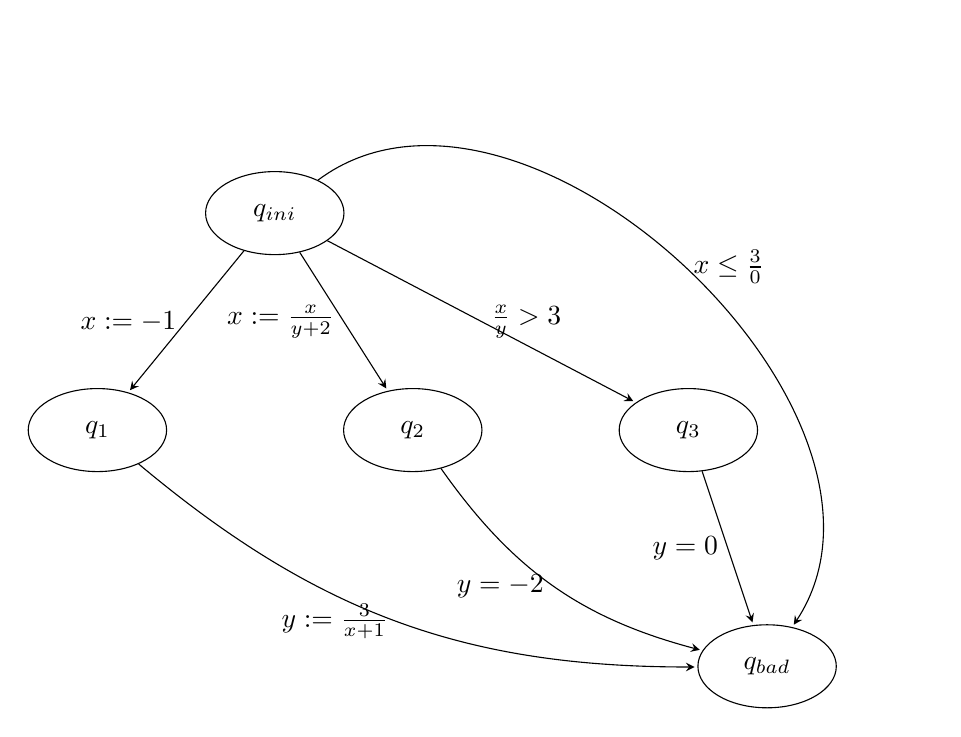
\begin{tikzpicture}[%
    ->,
    shorten >=1pt,
    >=stealth,
    node distance=7cm,
    noname/.style={%
      ellipse,
      minimum width=5em,
      minimum height=3em,
      draw
    }
  ]
    \node[noname] (ini)                                                {$q_{ini}$};
    \node[noname] (1) [node distance=2cm and 1cm,below left=of ini]    {$q_{1}$};
    \node[noname] (2) [node distance=2cm and 0.5cm,below right=of ini] {$q_{2}$};
    \node[noname] (3) [node distance=2cm and 4cm,below right=of ini]   {$q_{3}$};
    \node[noname] (bad) [node distance=5cm and 5cm,below right=of ini]   {$q_{bad}$};

    \path (ini) edge [left]                  node {$x:=-1$} (1)
          (ini) edge [left]                  node {$x:=\frac{x}{y+2}$} (2)
          (ini) edge [right]                  node {$\frac{x}{y} > 3$} (3)
          (ini) edge [bend left=80pt, right] node {$x \leq \frac{3}{0}$} (bad)
          (1)   edge [bend right=20pt, left] node {$y:=\frac{3}{x+1}$} (bad)
          (2)   edge [bend right=20pt, left] node {$y = -2$} (bad)
          (3)   edge [left] node {$y=0$} (bad)
          ;
  \end{tikzpicture}

\subsection{Constant Propagation}

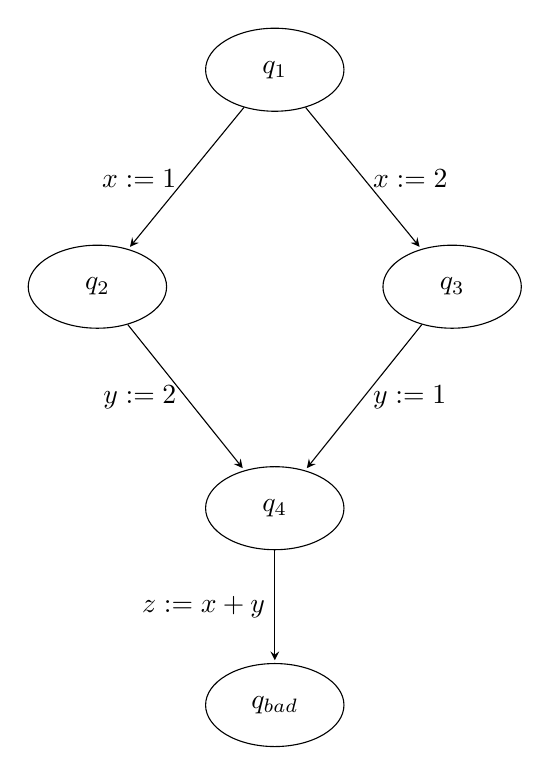
\begin{tikzpicture}[%
    ->,
    shorten >=1pt,
    >=stealth,
    node distance=7cm,
    noname/.style={%
      ellipse,
      minimum width=5em,
      minimum height=3em,
      draw
    }
  ]
    \node[noname] (1)                                                {$q_{1}$};
    \node[noname] (2) [node distance=2cm and 1cm,below left=of 1]    {$q_{2}$};
    \node[noname] (3) [node distance=2cm and 1cm,below right=of 1] {$q_{3}$};
    \node[noname] (4) [node distance=4.5cm,below =of 1]   {$q_{4}$};
    \node[noname] (bad) [node distance=7cm,below =of 1]   {$q_{bad}$};

    \path (1) edge [left]                   node {$x:=1$}   (2)
          (1) edge [right]                  node {$x:=2$}   (3)
          (2) edge [left]                   node {$y:=2$}   (4)
          (3) edge [right] 					node {$y:=1$}   (4)
          (4) edge [left]  					node {$z:=x+y$} (bad)
          ;
  \end{tikzpicture}

\subsection{Inductive Invariants Exercise 1}
\begin{tikzpicture}[%
    ->,
    shorten >=1pt,
    >=stealth,
    node distance=7cm,
    noname/.style={%
      ellipse,
      minimum width=5em,
      minimum height=3em,
      draw
    }
  ]
    \node[noname] (0)                                      {$q_{0}$};
    \node[noname] (1)   [node distance=3cm, right=of 0]    {$q_{1}$};
    \node[noname] (bad) [node distance=8cm, right=of 0]    {$q_{bad}$};

    \path (0) edge [above]                    node {$x:=0$}       (1)
          (1) edge [loop above=80pt,above]    node {$x:=(x*y)$}   (1)
          (1) edge [loop below=100pt, below]  node {$x:=(x+3)$}   (1)
          (1) edge [above]  				  node {$x==10$}     (bad)
          ;
  \end{tikzpicture}
  
\subsection{Inductive Invariants Exercise 2}

\begin{tikzpicture}[%
    ->,
    shorten >=1pt,
    >=stealth,
    node distance=7cm,
    noname/.style={%
      ellipse,
      minimum width=5em,
      minimum height=3em,
      draw
    }
  ]
    \node[noname] (0)                                                {$q_{0}$};
    \node[noname] (1) [node distance=2cm,right=of 0]    {$q_{1}$};
    \node[noname] (2) [node distance=2cm,right=of 1] {$q_{2}$};
    \node[noname] (3) [node distance=2cm,right=of 2]   {$q_{3}$};
    \node[noname] (4) [node distance=2cm,below=of 2]   {$q_{4}$};
    \node[noname, red] (bad) [node distance=2cm,left=of 4]   {$q_{bad}$};

    \path (ini) edge [above]                  node {$y > 0$} (1)
          (1) edge [above]                    node {$x:=0$} (2)
          (2) edge [bend right=20pt,below]     node {$x:= (x+y)$} (3)
          (2) edge [right]   node {$y==0$} (4)
          (3) edge [bend right=20pt, above]   node {$y:=(y-1)$} (2)
          (4) edge [above]   node {$x==0$} (bad)
          ;
  \end{tikzpicture}

\subsection{Running Example}
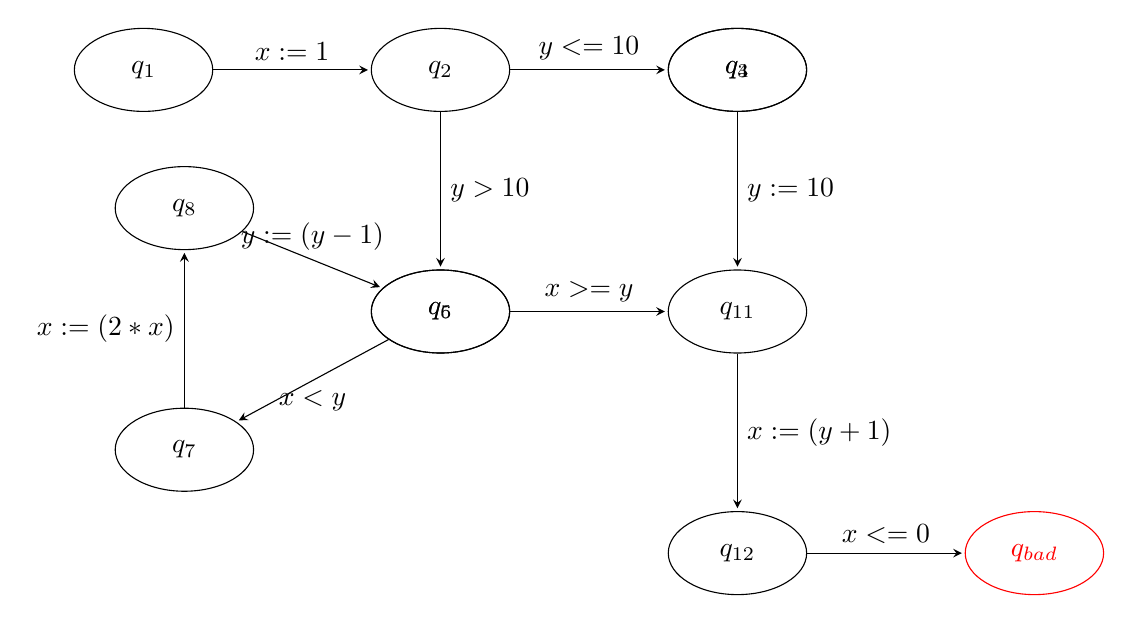
\begin{tikzpicture}[%
    ->,
    shorten >=1pt,
    >=stealth,
    node distance=7cm,
    noname/.style={%
      ellipse,
      minimum width=5em,
      minimum height=3em,
      draw
    }
  ]
    \node[noname] (1)                                   {$q_{1}$};
    \node[noname] (2) [node distance=2cm,right=of 1]    {$q_{2}$};
    \node[noname] (3) [node distance=2cm,right=of 2]    {$q_{3}$};
    \node[noname] (4) [node distance=2cm,right=of 2]    {$q_{4}$};
    \node[noname] (5) [node distance=2cm,below=of 2]    {$q_{5}$};
    \node[noname] (6) [node distance=2cm,below=of 2]    {$q_{6}$};
    \node[noname] (7) [node distance=1cm and 2cm,below left=of 6]    {$q_{7}$};
    \node[noname] (8) [node distance=2cm,above=of 7]    {$q_{8}$};
    \node[noname] (11) [node distance=2cm,below =of 3]   {$q_{11}$};
    \node[noname] (12) [node distance=2cm,below=of 11]   {$q_{12}$};
    \node[noname, red] (bad) [node distance=2cm,right=of 12]   {$q_{bad}$};

    \path (1) edge [above]                  node {$x:=1$} (2)
          (2) edge [above]                  node {$y<=10$} (3)
          (2) edge [right]                  node {$y>10$} (6)
          (3) edge [right]   node {$y:=10$} (11)
          (6) edge [below]   node {$x<y$} (7)
          (6) edge [above]   node {$x>=y$} (11) 
          (7) edge [left]   node {$x:=(2*x)$} (8)
          (8) edge [above]   node {$y:=(y-1)$} (6)
          (11) edge [right]   node {$x:= (y+1)$} (12)
          (12) edge [above]   node {$x<=0$} (bad)
          ;
  \end{tikzpicture}
\subsection{Infinite Descent}

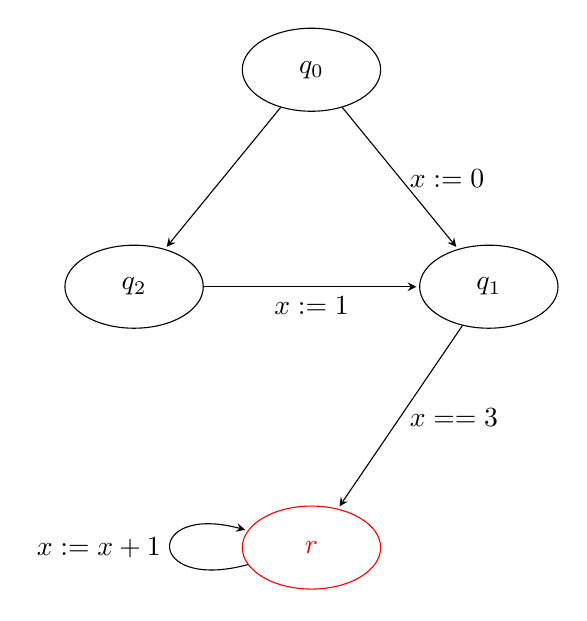
\begin{tikzpicture}[%
    ->,
    shorten >=1pt,
    >=stealth,
    node distance=7cm,
    noname/.style={%
      ellipse,
      minimum width=5em,
      minimum height=3em,
      draw
    }
  ]
    \node[noname] (0)                                                {$q_{0}$};
    \node[noname] (1) [node distance=2cm and 1cm,below right=of 0]   {$q_{1}$};
    \node[noname] (2) [node distance=2cm and 1cm,below left=of 0]    {$q_{2}$};
    \node[noname, red] (bad) [node distance=5cm,below=of 0]          {$r$};

    \path (0) edge []                    node {}       (2)
          (0) edge [right]                    node {$x:=0$} (1)
          (1) edge [right]    node {$x == 3$} (bad)
          (2) edge [below]                    node {$x:=1$} (1)
          (bad) edge [loop left]                    node {$x:=x+1$} (bad)
          ;
  \end{tikzpicture}

\subsection{Pre Only}

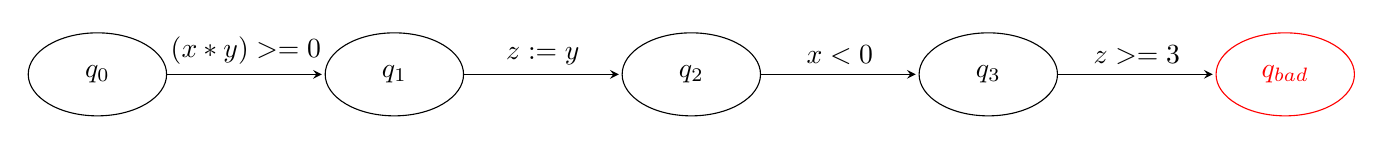
\begin{tikzpicture}[%
    ->,
    shorten >=1pt,
    >=stealth,
    node distance=7cm,
    noname/.style={%
      ellipse,
      minimum width=5em,
      minimum height=3em,
      draw
    }
  ]
    \node[noname] (0)                                                {$q_{0}$};
    \node[noname] (1) [node distance=2cm, right=of 0]   {$q_{1}$};
    \node[noname] (2) [node distance=2cm, right=of 1]    {$q_{2}$};
    \node[noname] (3) [node distance=2cm, right=of 2]    {$q_{3}$};
    \node[noname, red] (bad) [node distance=2cm,right=of 3]          {$q_{bad}$};

    \path (0) edge [above]                    node {$(x*y) >= 0$}       (1)
          (1) edge [above]                    node {$z:=y$} (2)
          (2) edge [above]                     node {$x<0$} (3)
          (3) edge [above]                    node {$z>=3$} (bad)
          ;
  \end{tikzpicture}

\subsection{Sign Non Zero Crucial}
\subsection{Sign Non Zero Crucial Variant}
\section{Implementation of BoundedModelChecking.ml}

\section{Conclusions}
\section{The Ocaml debugger}
Invoked via:
\begin{minted}{c}
ocamldebug bmc.d.byte
\end{minted}
Setting command line arguments:
\begin{minted}{c}
(ocd) set arguments examples/constant_propagation.aut
(ocd) break @BoundedModelChecking 87
\end{minted}




Here you briefly summarize your findings.

%++++++++++++++++++++++++++++++++++++++++
% References section will be created automatically 
% with inclusion of "thebibliography" environment
% as it shown below. See text starting with line
% \begin{thebibliography}{99}
% Note: with this approach it is YOUR responsibility to put them in order
% of appearance.

\begin{thebibliography}{99}

\bibitem{melissinos}
A.~C. Melissinos and J. Napolitano, \textit{Experiments in Modern Physics},
(Academic Press, New York, 2003).

\bibitem{Cyr}
N.\ Cyr, M.\ T$\hat{e}$tu, and M.\ Breton,
% "All-optical microwave frequency standard: a proposal,"
IEEE Trans.\ Instrum.\ Meas.\ \textbf{42}, 640 (1993).

\bibitem{Wiki} \emph{Expected value},  available at
\texttt{http://en.wikipedia.org/wiki/Expected\_value}.

\end{thebibliography}


\end{document}
